\documentclass[border=8pt]{standalone}
\usepackage{tikz}
\usepackage{amsmath,amssymb}
\usetikzlibrary{arrows.meta, positioning, calc, fit, backgrounds}

\definecolor{accent}{HTML}{1B4F72}
\definecolor{accentdeep}{HTML}{0E2F44}
\definecolor{accentmid}{HTML}{2E86C1}
\definecolor{accentlight}{HTML}{EBF5FB}
\definecolor{gold}{HTML}{D4AC0D}
\definecolor{goldlight}{HTML}{FFF8DC}
\definecolor{bordersoft}{HTML}{BDC3C7}
\definecolor{frozenblock}{HTML}{E8E8E8}
\definecolor{textmuted}{HTML}{888888}

\begin{document}
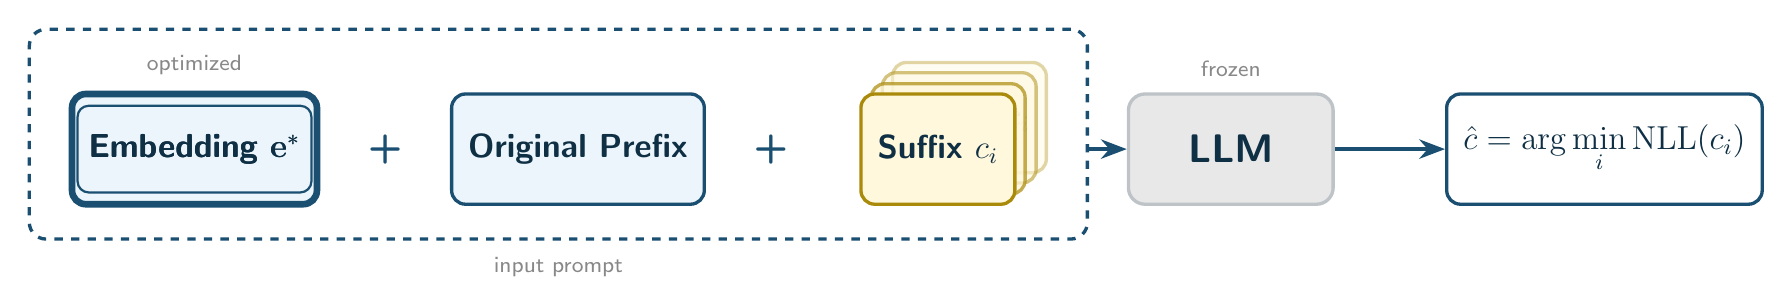
\begin{tikzpicture}[
    >=Stealth,
    font=\sffamily,
    every node/.style={inner sep=0pt},
    mainbox/.style={
        draw=accent, line width=1.2pt, rounded corners=5pt,
        fill=accentlight, minimum height=14mm,
        font=\sffamily\bfseries\large, text=accentdeep, align=center,
        inner sep=6pt
    },
    embbox/.style={
        draw=accent, line width=2.4pt, rounded corners=5pt,
        fill=accentlight, minimum height=14mm,
        font=\sffamily\bfseries\large, text=accentdeep, align=center,
        inner sep=6pt
    },
    suffbox/.style={
        draw=gold!80!black, line width=1.2pt, rounded corners=5pt,
        fill=goldlight, minimum height=14mm,
        font=\sffamily\bfseries\large, text=accentdeep, align=center,
        inner sep=6pt
    },
    llmbox/.style={
        draw=bordersoft, line width=1.2pt, rounded corners=6pt,
        fill=frozenblock, minimum height=14mm, minimum width=26mm,
        font=\sffamily\bfseries\Large, text=accentdeep, align=center,
        inner sep=6pt
    },
    resultbox/.style={
        draw=accent, line width=1.2pt, rounded corners=5pt,
        fill=white, minimum height=14mm,
        font=\sffamily\large, text=accentdeep, align=center,
        inner sep=6pt
    },
    arrstyle/.style={->, line width=1.4pt, accent},
    pluslabel/.style={font=\sffamily\bfseries\Large, text=accent},
    mlabel/.style={font=\sffamily\footnotesize, text=textmuted},
]

% === Embedding e* ===
\node[embbox] (emb) {Embedding $\mathbf{e}^*$};
% inner double border
\node[draw=accent, line width=0.8pt, rounded corners=4pt,
      minimum height=11mm, inner sep=4pt,
      font=\sffamily\bfseries\large, text=accentdeep] at (emb.center) {Embedding $\mathbf{e}^*$};
\node[mlabel, above=2mm of emb] {optimized};

% === Plus ===
\node[pluslabel, right=6mm of emb] (p1) {+};

% === Original Prefix ===
\node[mainbox, right=6mm of p1] (prefix) {Original Prefix};

% === Plus ===
\node[pluslabel, right=6mm of prefix] (p2) {+};

% === Suffix stack (×4 behind) ===
% back copies for stacking effect
\node[suffbox, right=9mm of p2, xshift=4mm, yshift=4mm, opacity=0.35] (s4) {Suffix $c_i$};
\node[suffbox, right=9mm of p2, xshift=2.7mm, yshift=2.7mm, opacity=0.5] (s3) {Suffix $c_i$};
\node[suffbox, right=9mm of p2, xshift=1.3mm, yshift=1.3mm, opacity=0.7] (s2) {Suffix $c_i$};
% front copy
\node[suffbox, right=9mm of p2] (suf) {Suffix $c_i$};

% === Arrow to LLM ===
\node[llmbox, right=14mm of suf] (llm) {LLM};
\node[mlabel, above=2mm of llm] {frozen};

% === Result ===
\node[resultbox, right=14mm of llm] (res) {$\hat{c} = \arg\min\limits_i \mathrm{NLL}(c_i)$};

% === Dashed surrounding rectangle for all prompt blocks ===
\begin{pgfonlayer}{background}
\node[draw=accent, line width=1.2pt, dashed, rounded corners=6pt,
      fill=white, fill opacity=0.3,
      inner xsep=5mm, inner ysep=4mm,
      fit=(emb)(s4)(p1)(prefix)(p2)(suf)] (promptgroup) {};
\end{pgfonlayer}
\node[mlabel, below=2mm of promptgroup] {input prompt};

% === Arrows ===
\draw[arrstyle] (promptgroup.east |- llm.west) -- (llm.west);
\draw[arrstyle] (llm.east) -- (res.west);

\end{tikzpicture}
\end{document}
